\documentclass[12pt]{article}

% TEMPLATE DEFAULT PACKAGES
\usepackage{amssymb,amsmath,amsfonts,eurosym,geometry,ulem,graphicx,color,setspace,sectsty,comment,natbib,pdflscape,array,adjustbox}

% ADDED PACKAGES FOR THIS MANUSCRIPT
\usepackage{palatino,newtxmath,multirow,titlesec,threeparttable,tabu,booktabs,titlesec,threeparttable,mathtools,bm,bbm,subcaption,pdflscape,tcolorbox,mathrsfs}
% endfloat,

\usepackage{afterpage}
\usepackage[hyphens]{url}
\usepackage[margin=1cm]{caption}

\usepackage[draft]{hyperref}
\newcommand{\tim}{$\,\times\,$}
% FIGURES & TABLES CAPTION STYLING
\captionsetup[figure]{labelfont={bf},name={Figure},labelsep=period}
\captionsetup[table]{labelfont={bf},name={Table},labelsep=period}

% SECTION TITLE SETTINGS
\titlelabel{\thetitle.\enskip}
\titleformat*{\section}{\large\bfseries}
\titleformat*{\subsection}{\normalsize\bfseries}

% COLUMN TYPES
\newcolumntype{L}[1]{>{\raggedright\let\newline\\\arraybackslash\hspace{0pt}}m{#1}}
\newcolumntype{C}{>{\centering\arraybackslash}p{5.2em}}
\newcolumntype{D}{>{\centering\arraybackslash}p{5em}}
\newcolumntype{R}[1]{>{\raggedleft\let\newline\\\arraybackslash\hspace{0pt}}m{#1}}


% MARGINS AND SPACING
\normalem
\geometry{left=1.1in,right=1.1in,top=1.0in,bottom=1.0in}
\setlength{\parskip}{2.5pt}

% SPECIAL CELL 
\newcommand{\specialcell}[2][c]{%
	\begin{tabular}[#1]{@{}l@{}}#2\end{tabular}}

% NO INDENT ON FOOTNOTES
\usepackage[hang,flushmargin]{footmisc}

\begin{document}


\begin{table}
\caption{Building Density}
\begin{tabular}{lDDDD}
\toprule
 & \small (1)  & \small (2) & \small (3) & \small (4) \\
 & Total & Formal   & Informal Bkyd. & Informal Non-Bkyd. \\ \midrule
inside project      &     611.592\textsuperscript{a}&     620.033\textsuperscript{a}&      -8.441                   &     521.964\textsuperscript{a}&    -530.405\textsuperscript{a}\\
                    &   (191.184)                   &    (98.725)                   &   (139.037)                   &   (124.975)                   &   (131.385)                   \\[0.55em]
0-500m outside project &    -189.479\textsuperscript{c}&     -28.176                   &    -161.303\textsuperscript{b}&     -95.671                   &     -65.632                   \\
                    &    (98.595)                   &    (54.169)                   &    (82.296)                   &    (71.083)                   &    (69.985)                   \\[0.5em]
Mean Outcome 2001   &      524.85                   &      261.16                   &      263.69                   &       96.38                   &      167.31                   \\
Mean Outcome 2011   &      836.05                   &      384.05                   &      452.00                   &      286.03                   &      165.98                   \\
R$^2$               &       0.305                   &       0.276                   &       0.263                   &       0.189                   &       0.259                   \\
\# projects         &         316                   &         316                   &         316                   &         316                   &         316                   \\
N project areas     &     586,918                   &     586,918                   &     586,918                   &     586,918                   &     586,918                   \\
N spillover areas   &   1,080,542                   &   1,080,542                   &   1,080,542                   &   1,080,542                   &   1,080,542                   \\
N                   &   6,822,716                   &   6,822,716                   &   6,822,716                   &   6,822,716                   &   6,822,716                   \\

\midrule
% \textbf{Low Income} \\  inside project      &     517.311\textsuperscript{c}&     652.122\textsuperscript{a}&     609.262\textsuperscript{a}&    -744.073\textsuperscript{a}\\
                    &   (264.611)                   &   (112.777)                   &   (158.618)                   &   (218.154)                   \\[0.02em]
0-500m outside project &    -166.300                   &       2.496                   &    -162.468                   &      -6.329                   \\
                    &   (145.863)                   &    (96.651)                   &   (129.158)                   &   (113.193)                   \\[0.55em]
\textbf{High Income} \\  inside project      &     589.805\textsuperscript{b}&     590.147\textsuperscript{a}&     198.668                   &    -199.010\textsuperscript{b}\\
                    &   (260.891)                   &   (158.503)                   &   (122.642)                   &    (98.479)                   \\[0.02em]
0-500m outside project &    -258.734\textsuperscript{c}&     -82.837                   &     -78.539                   &     -97.357                   \\
                    &   (144.483)                   &    (55.705)                   &    (61.077)                   &    (81.255)                   \\[0.55em]
Mean                &      680.45                   &      322.61                   &      191.20                   &      166.64                   \\
N                   &   6,822,716                   &   6,822,716                   &   6,822,716                   &   6,822,716                   \\

% \bottomrule
\end{tabular}
\end{table}



\begin{table}
\caption{Building Density by Neighborhood Income Quartile}
\begin{tabular}{lDDDD}
\toprule
 & \small (1)  & \small (2) & \small (3) & \small (4) \\
 & Total & Formal   & Informal Bkyd. & Informal Non-Bkyd. \\ \midrule
Q1: inside project  &     158.786                   &     645.656\textsuperscript{a}&    -486.870                   &   -1076.663\textsuperscript{a}&     589.793\textsuperscript{a}\\
                    &   (332.489)                   &   (148.783)                   &   (295.986)                   &   (318.545)                   &   (205.212)                   \\[.2em]
Q1: 0-500m outside project &    -127.239                   &     -53.468                   &     -73.771                   &      20.876                   &     -94.646                   \\
                    &   (200.414)                   &   (159.558)                   &   (187.859)                   &   (202.674)                   &   (186.594)                   \\[.5em]
Q2: inside project  &    1072.658\textsuperscript{b}&     641.216\textsuperscript{a}&     431.442                   &    -181.306                   &     612.748\textsuperscript{b}\\
                    &   (456.610)                   &   (189.734)                   &   (297.703)                   &   (129.887)                   &   (287.505)                   \\[.2em]
Q2: 0-500m outside project &    -348.734                   &      51.902                   &    -400.636                   &      -9.340                   &    -391.296\textsuperscript{c}\\
                    &   (256.546)                   &    (41.531)                   &   (246.177)                   &    (60.775)                   &   (228.942)                   \\[.5em]
Q3: inside project  &     546.381\textsuperscript{b}&     652.869\textsuperscript{a}&    -106.488                   &    -380.784\textsuperscript{b}&     274.297\textsuperscript{a}\\
                    &   (272.069)                   &   (197.426)                   &   (199.100)                   &   (171.097)                   &    (97.758)                   \\[.2em]
Q3: 0-500m outside project &    -391.067\textsuperscript{b}&    -176.028\textsuperscript{c}&    -215.039\textsuperscript{c}&     -59.031                   &    -156.008                   \\
                    &   (195.362)                   &   (100.938)                   &   (126.066)                   &    (80.438)                   &   (103.811)                   \\[.5em]
Q4: inside project  &     524.434                   &     497.350\textsuperscript{c}&      27.084                   &     -88.771                   &     115.855                   \\
                    &   (518.930)                   &   (253.939)                   &   (302.993)                   &    (64.540)                   &   (267.761)                   \\[.2em]
Q4: 0-500m outside project &    -245.420                   &     -21.493                   &    -223.927                   &    -169.971                   &     -53.956                   \\
                    &   (266.217)                   &    (83.955)                   &   (190.562)                   &   (163.233)                   &    (81.636)                   \\[.5em]
Mean Pre            &      579.36                   &      288.49                   &      290.87                   &      184.19                   &      106.68                   \\
Mean Post           &      922.93                   &      424.41                   &      498.52                   &      182.46                   &      316.06                   \\
R$^2$               &       0.323                   &       0.294                   &       0.278                   &       0.274                   &       0.205                   \\
N                   &   6,143,756                   &   6,143,756                   &   6,143,756                   &   6,143,756                   &   6,143,756                   \\

\midrule
% \textbf{Low Income} \\  inside project      &     517.311\textsuperscript{c}&     652.122\textsuperscript{a}&     609.262\textsuperscript{a}&    -744.073\textsuperscript{a}\\
                    &   (264.611)                   &   (112.777)                   &   (158.618)                   &   (218.154)                   \\[0.02em]
0-500m outside project &    -166.300                   &       2.496                   &    -162.468                   &      -6.329                   \\
                    &   (145.863)                   &    (96.651)                   &   (129.158)                   &   (113.193)                   \\[0.55em]
\textbf{High Income} \\  inside project      &     589.805\textsuperscript{b}&     590.147\textsuperscript{a}&     198.668                   &    -199.010\textsuperscript{b}\\
                    &   (260.891)                   &   (158.503)                   &   (122.642)                   &    (98.479)                   \\[0.02em]
0-500m outside project &    -258.734\textsuperscript{c}&     -82.837                   &     -78.539                   &     -97.357                   \\
                    &   (144.483)                   &    (55.705)                   &    (61.077)                   &    (81.255)                   \\[0.55em]
Mean                &      680.45                   &      322.61                   &      191.20                   &      166.64                   \\
N                   &   6,822,716                   &   6,822,716                   &   6,822,716                   &   6,822,716                   \\

% \bottomrule
\end{tabular}
\end{table}


\begin{table}[]
\small
\centering
\caption{Census Household-level Estimates}\label{table:censusestimates}
\vspace{-2mm}
\begin{tabular}{lDDDDDD}
\toprule
 & \small (1) & \small (2)  & \small (3) & \small (4)  & \small (5) & \small (6) \\
 & \small Formal House & \small Flush Toilet & \small Water Indoors  & \small Electricity & \small Total Rooms  & \small Own House  \\ \midrule
inside project      &       0.298\textsuperscript{b}&       0.063                   &      -0.143                   &      -0.031                   &    2584.083\textsuperscript{b}\\
                    &     (0.132)                   &     (0.185)                   &     (0.239)                   &     (1.577)                   &  (1278.139)                   \\[0.55em]
0-500m outside      &       0.025                   &      -0.115                   &      -0.074                   &      -0.145                   &     175.090                   \\
                    &     (0.092)                   &     (0.080)                   &     (0.089)                   &     (0.397)                   &   (736.878)                   \\[0.5em]
Mean Pre            &        0.47                   &        0.71                   &        0.70                   &        3.48                   &    1,793.45                   \\
Mean Post           &        0.54                   &        0.77                   &        0.77                   &        3.79                   &    2,690.42                   \\
R$^2$               &       0.577                   &       0.612                   &       0.574                   &       0.587                   &       0.551                   \\
N                   &      20,639                   &      20,639                   &      20,639                   &      20,500                   &      21,197                   \\
 \midrule
 \\
 & \small (5)  & \small (6)  & \small (7) & \small (8)  & \small (9)  & \small (10)\\
 & \small HH Size & Total People & Age HoH & African HoH & Employed HoH & HH Log Income \\ \midrule
inside project      &       0.845\textsuperscript{a}&      -0.004                   &       0.301\textsuperscript{b}&    -513.215                   \\
                    &     (0.296)                   &     (0.119)                   &     (0.129)                   &   (594.289)                   \\[0.55em]
0-500m outside project &       0.012                   &       0.030                   &       0.121                   &    -120.124                   \\
                    &     (0.170)                   &     (0.046)                   &     (0.085)                   &   (424.193)                   \\[0.5em]
Mean Pre            &        3.22                   &        0.69                   &        3.72                   &   10,530.22                   \\
Mean Post           &        3.59                   &        0.46                   &        3.24                   &   10,079.44                   \\
R$^2$               &       0.666                   &       0.418                   &       0.573                   &       0.725                   \\
N                   &      19,940                   &      20,063                   &      19,947                   &      20,524                   \\

% project{\tim}post{\tim}constr&       0.115\textsuperscript{c}&       0.164\textsuperscript{a}&       0.259\textsuperscript{a}&       0.181\textsuperscript{a}&       0.066                   &      -0.074                   &      -0.266\textsuperscript{b}&      99.563                   \\
            &     (0.069)                   &     (0.050)                   &     (0.072)                   &     (0.066)                   &     (0.084)                   &     (0.173)                   &     (0.107)                   &  (1448.879)                   \\[0.5em]
project{\tim}post&       0.064                   &       0.090\textsuperscript{b}&       0.176\textsuperscript{a}&       0.151\textsuperscript{a}&       0.144\textsuperscript{b}&       0.408\textsuperscript{a}&      -0.039                   &    2320.431\textsuperscript{b}\\
            &     (0.046)                   &     (0.039)                   &     (0.060)                   &     (0.055)                   &     (0.066)                   &     (0.129)                   &     (0.056)                   &  (1111.722)                   \\[0.5em]
project{\tim}constr&       0.070                   &      -0.024                   &      -0.066                   &      -0.061                   &       0.129                   &       0.195                   &       0.460\textsuperscript{a}&    -611.013                   \\
            &     (0.111)                   &     (0.090)                   &     (0.105)                   &     (0.093)                   &     (0.125)                   &     (0.284)                   &     (0.128)                   &  (1733.494)                   \\[0.5em]
project     &      -0.321\textsuperscript{a}&      -0.239\textsuperscript{a}&      -0.354\textsuperscript{a}&      -0.320\textsuperscript{a}&      -0.362\textsuperscript{a}&      -1.065\textsuperscript{a}&      -0.403\textsuperscript{a}&     416.265                   \\
            &     (0.077)                   &     (0.053)                   &     (0.069)                   &     (0.064)                   &     (0.080)                   &     (0.175)                   &     (0.082)                   &   (691.463)                   \\[0.5em]
spillover{\tim}post{\tim}constr&       0.013                   &       0.045                   &       0.028                   &      -0.037                   &      -0.038                   &       0.053                   &      -0.153\textsuperscript{a}&     444.064                   \\
            &     (0.034)                   &     (0.033)                   &     (0.034)                   &     (0.043)                   &     (0.027)                   &     (0.078)                   &     (0.049)                   &   (470.258)                   \\[0.5em]
spillover{\tim}post&       0.039                   &       0.133\textsuperscript{a}&       0.101\textsuperscript{a}&       0.082\textsuperscript{a}&       0.058\textsuperscript{b}&       0.249\textsuperscript{a}&      -0.156\textsuperscript{a}&     652.913\textsuperscript{b}\\
            &     (0.024)                   &     (0.028)                   &     (0.024)                   &     (0.023)                   &     (0.023)                   &     (0.055)                   &     (0.036)                   &   (325.594)                   \\[0.5em]
spillover{\tim}constr&      -0.029                   &      -0.056                   &      -0.065                   &      -0.041                   &       0.015                   &      -0.252\textsuperscript{c}&       0.143\textsuperscript{b}&     -23.442                   \\
            &     (0.049)                   &     (0.055)                   &     (0.044)                   &     (0.042)                   &     (0.050)                   &     (0.145)                   &     (0.059)                   &  (1353.816)                   \\ \midrule
{\it p}-val, h\textsubscript{0}: project=spill. &       0.119                   &       0.029                   &       0.001                   &       0.001                   &       0.208                   &       0.439                   &       0.250                   &       0.811                   \\
Mean Outcome 2001&        0.72                   &        0.31                   &        0.60                   &        0.57                   &        0.75                   &        3.31                   &        3.59                   &    7,313.26                   \\
Mean Outcome 2011&        0.79                   &        0.51                   &        0.80                   &        0.69                   &        0.82                   &        3.57                   &        3.22                   &    9,118.36                   \\
R$^2$       &       0.336                   &       0.318                   &       0.363                   &       0.315                   &       0.294                   &       0.368                   &       0.443                   &       0.398                   \\
\# projects &         117                   &         117                   &         117                   &         117                   &         117                   &         117                   &         117                   &         117                   \\
N project areas&       3,631                   &       3,631                   &       3,631                   &       3,631                   &       3,631                   &       3,630                   &       3,632                   &       3,632                   \\
N spillover areas&       5,978                   &       5,978                   &       5,978                   &       5,978                   &       5,978                   &       5,964                   &       5,977                   &       5,980                   \\
N           &       9,609                   &       9,609                   &       9,609                   &       9,609                   &       9,609                   &       9,594                   &       9,609                   &       9,612                   \\

\bottomrule\\[-.6em]
\multicolumn{7}{l}{\footnotesize Standard errors clustered at the project level in parenthesis.\textsuperscript{c} p$<$0.10,\textsuperscript{b} p$<$0.05,\textsuperscript{a} p$<$0.01} \\[-.3em] 
\multicolumn{7}{l}{\footnotesize Specifications include census 2001 subplace fixed effects.} \\[-.3em] 
\multicolumn{7}{l}{\footnotesize Results are weighted by unit area and control for up to a cubic in unit area by time. }
\end{tabular}
\end{table}


\begin{table}[]
\small
\centering
\caption{Census Household-level Estimates in Spillover Area by Neighborhood Income Quartile}\label{table:censusestimatesinc}
\vspace{-2mm}
\begin{tabular}{lDDDDDD}
\toprule
 & \small (1) & \small (2)  & \small (3) & \small (4)  & \small (5) & \small (6) \\
 & \small Formal House & \small Flush Toilet & \small Water Indoors  & \small Electricity & \small Total Rooms  & \small Own House  \\ \midrule
Q1: inside project  &       0.522\textsuperscript{b}&       0.850\textsuperscript{a}&       0.634\textsuperscript{a}&       0.816\textsuperscript{a}&       1.313\textsuperscript{b}&       0.024                   \\
                    &     (0.223)                   &     (0.173)                   &     (0.156)                   &     (0.261)                   &     (0.513)                   &     (0.194)                   \\[.2em]
Q1: 0-500m outside project &       0.193                   &      -0.153                   &       0.326                   &       0.102                   &       0.080                   &       0.386\textsuperscript{b}\\
                    &     (0.226)                   &     (0.310)                   &     (0.248)                   &     (0.144)                   &     (0.551)                   &     (0.168)                   \\[.5em]
Q2: inside project  &       0.036                   &       0.202                   &      -0.039                   &      -0.129                   &      -0.853\textsuperscript{b}&       0.120                   \\
                    &     (0.093)                   &     (0.235)                   &     (0.117)                   &     (0.317)                   &     (0.411)                   &     (0.118)                   \\[.2em]
Q2: 0-500m outside project &      -0.125                   &      -0.169                   &      -0.248                   &      -0.158                   &      -0.923                   &      -0.309\textsuperscript{c}\\
                    &     (0.240)                   &     (0.166)                   &     (0.239)                   &     (0.183)                   &     (0.915)                   &     (0.181)                   \\[.5em]
Q3: inside project  &       0.218\textsuperscript{a}&      -0.034                   &       0.067\textsuperscript{b}&       0.188                   &       0.220                   &      -0.368\textsuperscript{a}\\
                    &     (0.059)                   &     (0.183)                   &     (0.032)                   &     (0.183)                   &     (0.430)                   &     (0.079)                   \\[.2em]
Q3: 0-500m outside project &       0.023                   &      -0.008                   &      -0.157                   &      -0.074                   &      -0.754\textsuperscript{b}&      -0.006                   \\
                    &     (0.124)                   &     (0.072)                   &     (0.147)                   &     (0.095)                   &     (0.384)                   &     (0.124)                   \\[.5em]
Q4: inside project  &      -0.399\textsuperscript{a}&       0.566\textsuperscript{a}&       0.259                   &       0.600\textsuperscript{a}&      -0.398                   &      -0.800\textsuperscript{a}\\
                    &     (0.143)                   &     (0.150)                   &     (0.205)                   &     (0.174)                   &     (0.603)                   &     (0.124)                   \\[.2em]
Q4: 0-500m outside project &      -0.201                   &      -0.171\textsuperscript{c}&       0.024                   &      -0.105                   &       1.868\textsuperscript{a}&       0.330                   \\
                    &     (0.256)                   &     (0.088)                   &     (0.186)                   &     (0.097)                   &     (0.688)                   &     (0.304)                   \\[.5em]
Mean Pre            &        0.62                   &        0.71                   &        0.47                   &        0.70                   &        3.48                   &        0.41                   \\
Mean Post           &        0.65                   &        0.77                   &        0.54                   &        0.77                   &        3.79                   &        0.36                   \\
R$^2$               &       0.578                   &       0.650                   &       0.612                   &       0.625                   &       0.653                   &       0.613                   \\
N                   &      20,641                   &      20,639                   &      20,639                   &      20,639                   &      20,500                   &      20,631                   \\
 \midrule
% project{\tim}post{\tim}constr&       0.115\textsuperscript{c}&       0.164\textsuperscript{a}&       0.259\textsuperscript{a}&       0.181\textsuperscript{a}&       0.066                   &      -0.074                   &      -0.266\textsuperscript{b}&      99.563                   \\
            &     (0.069)                   &     (0.050)                   &     (0.072)                   &     (0.066)                   &     (0.084)                   &     (0.173)                   &     (0.107)                   &  (1448.879)                   \\[0.5em]
project{\tim}post&       0.064                   &       0.090\textsuperscript{b}&       0.176\textsuperscript{a}&       0.151\textsuperscript{a}&       0.144\textsuperscript{b}&       0.408\textsuperscript{a}&      -0.039                   &    2320.431\textsuperscript{b}\\
            &     (0.046)                   &     (0.039)                   &     (0.060)                   &     (0.055)                   &     (0.066)                   &     (0.129)                   &     (0.056)                   &  (1111.722)                   \\[0.5em]
project{\tim}constr&       0.070                   &      -0.024                   &      -0.066                   &      -0.061                   &       0.129                   &       0.195                   &       0.460\textsuperscript{a}&    -611.013                   \\
            &     (0.111)                   &     (0.090)                   &     (0.105)                   &     (0.093)                   &     (0.125)                   &     (0.284)                   &     (0.128)                   &  (1733.494)                   \\[0.5em]
project     &      -0.321\textsuperscript{a}&      -0.239\textsuperscript{a}&      -0.354\textsuperscript{a}&      -0.320\textsuperscript{a}&      -0.362\textsuperscript{a}&      -1.065\textsuperscript{a}&      -0.403\textsuperscript{a}&     416.265                   \\
            &     (0.077)                   &     (0.053)                   &     (0.069)                   &     (0.064)                   &     (0.080)                   &     (0.175)                   &     (0.082)                   &   (691.463)                   \\[0.5em]
spillover{\tim}post{\tim}constr&       0.013                   &       0.045                   &       0.028                   &      -0.037                   &      -0.038                   &       0.053                   &      -0.153\textsuperscript{a}&     444.064                   \\
            &     (0.034)                   &     (0.033)                   &     (0.034)                   &     (0.043)                   &     (0.027)                   &     (0.078)                   &     (0.049)                   &   (470.258)                   \\[0.5em]
spillover{\tim}post&       0.039                   &       0.133\textsuperscript{a}&       0.101\textsuperscript{a}&       0.082\textsuperscript{a}&       0.058\textsuperscript{b}&       0.249\textsuperscript{a}&      -0.156\textsuperscript{a}&     652.913\textsuperscript{b}\\
            &     (0.024)                   &     (0.028)                   &     (0.024)                   &     (0.023)                   &     (0.023)                   &     (0.055)                   &     (0.036)                   &   (325.594)                   \\[0.5em]
spillover{\tim}constr&      -0.029                   &      -0.056                   &      -0.065                   &      -0.041                   &       0.015                   &      -0.252\textsuperscript{c}&       0.143\textsuperscript{b}&     -23.442                   \\
            &     (0.049)                   &     (0.055)                   &     (0.044)                   &     (0.042)                   &     (0.050)                   &     (0.145)                   &     (0.059)                   &  (1353.816)                   \\ \midrule
{\it p}-val, h\textsubscript{0}: project=spill. &       0.119                   &       0.029                   &       0.001                   &       0.001                   &       0.208                   &       0.439                   &       0.250                   &       0.811                   \\
Mean Outcome 2001&        0.72                   &        0.31                   &        0.60                   &        0.57                   &        0.75                   &        3.31                   &        3.59                   &    7,313.26                   \\
Mean Outcome 2011&        0.79                   &        0.51                   &        0.80                   &        0.69                   &        0.82                   &        3.57                   &        3.22                   &    9,118.36                   \\
R$^2$       &       0.336                   &       0.318                   &       0.363                   &       0.315                   &       0.294                   &       0.368                   &       0.443                   &       0.398                   \\
\# projects &         117                   &         117                   &         117                   &         117                   &         117                   &         117                   &         117                   &         117                   \\
N project areas&       3,631                   &       3,631                   &       3,631                   &       3,631                   &       3,631                   &       3,630                   &       3,632                   &       3,632                   \\
N spillover areas&       5,978                   &       5,978                   &       5,978                   &       5,978                   &       5,978                   &       5,964                   &       5,977                   &       5,980                   \\
N           &       9,609                   &       9,609                   &       9,609                   &       9,609                   &       9,609                   &       9,594                   &       9,609                   &       9,612                   \\

\bottomrule\\[-.6em]
\multicolumn{7}{l}{\footnotesize Standard errors clustered at the project level in parenthesis.\textsuperscript{c} p$<$0.10,\textsuperscript{b} p$<$0.05,\textsuperscript{a} p$<$0.01} \\[-.3em] 
\multicolumn{7}{l}{\footnotesize Specifications include census 2001 subplace fixed effects.} \\[-.3em] 
\multicolumn{7}{l}{\footnotesize Results are weighted by unit area and control for up to a cubic in unit area by time. }
\end{tabular}
\end{table}

\begin{table}[]
\small
\centering
\caption{Census Household-level Estimates in Spillover Area by Neighborhood Income Quartile}\label{table:censusestimatesinc2}
\vspace{-2mm}
\begin{tabular}{lDDDDDD}
\toprule
 & \small (5)  & \small (6)  & \small (7) & \small (8)  & \small (9)  & \small (10)\\
 & \small HH Size & Total People & Age HoH & African HoH & Employed HoH & HH Log Income \\ \midrule
Q1                  &      -0.092                   &   -1327.780                   &      -5.526\textsuperscript{b}&       0.068\textsuperscript{c}&      -0.218\textsuperscript{a}&      -0.664\textsuperscript{a}\\
                    &     (0.141)                   &  (1090.365)                   &     (2.482)                   &     (0.038)                   &     (0.051)                   &     (0.251)                   \\[.3em]
Q2                  &       0.005                   &     987.123                   &      -4.851                   &       0.061                   &      -0.125                   &      -1.180\textsuperscript{a}\\
                    &     (0.283)                   &  (1952.546)                   &     (3.084)                   &     (0.079)                   &     (0.086)                   &     (0.322)                   \\[.3em]
Q3                  &       0.654\textsuperscript{a}&   -1127.624                   &       0.947                   &       0.076\textsuperscript{b}&      -0.062                   &      -0.926\textsuperscript{a}\\
                    &     (0.159)                   &  (2360.625)                   &     (1.338)                   &     (0.035)                   &     (0.038)                   &     (0.130)                   \\[.3em]
Q4                  &       1.109\textsuperscript{a}&  -10377.097\textsuperscript{b}&       6.615\textsuperscript{b}&      -0.494\textsuperscript{a}&       0.091                   &       0.637\textsuperscript{a}\\
                    &     (0.309)                   &  (5173.586)                   &     (3.197)                   &     (0.167)                   &     (0.070)                   &     (0.233)                   \\[.3em]
Mean Pre            &        3.25                   &    1,793.45                   &       41.26                   &        0.73                   &        0.82                   &        7.30                   \\
Mean Post           &        2.89                   &    2,690.42                   &       42.34                   &        0.81                   &        0.83                   &        8.25                   \\
R$^2$               &       0.731                   &       0.583                   &       0.608                   &       0.740                   &       0.599                   &       0.698                   \\
N                   &      20,509                   &      21,197                   &      20,505                   &      20,641                   &      20,501                   &      20,495                   \\

% project{\tim}post{\tim}constr&       0.115\textsuperscript{c}&       0.164\textsuperscript{a}&       0.259\textsuperscript{a}&       0.181\textsuperscript{a}&       0.066                   &      -0.074                   &      -0.266\textsuperscript{b}&      99.563                   \\
            &     (0.069)                   &     (0.050)                   &     (0.072)                   &     (0.066)                   &     (0.084)                   &     (0.173)                   &     (0.107)                   &  (1448.879)                   \\[0.5em]
project{\tim}post&       0.064                   &       0.090\textsuperscript{b}&       0.176\textsuperscript{a}&       0.151\textsuperscript{a}&       0.144\textsuperscript{b}&       0.408\textsuperscript{a}&      -0.039                   &    2320.431\textsuperscript{b}\\
            &     (0.046)                   &     (0.039)                   &     (0.060)                   &     (0.055)                   &     (0.066)                   &     (0.129)                   &     (0.056)                   &  (1111.722)                   \\[0.5em]
project{\tim}constr&       0.070                   &      -0.024                   &      -0.066                   &      -0.061                   &       0.129                   &       0.195                   &       0.460\textsuperscript{a}&    -611.013                   \\
            &     (0.111)                   &     (0.090)                   &     (0.105)                   &     (0.093)                   &     (0.125)                   &     (0.284)                   &     (0.128)                   &  (1733.494)                   \\[0.5em]
project     &      -0.321\textsuperscript{a}&      -0.239\textsuperscript{a}&      -0.354\textsuperscript{a}&      -0.320\textsuperscript{a}&      -0.362\textsuperscript{a}&      -1.065\textsuperscript{a}&      -0.403\textsuperscript{a}&     416.265                   \\
            &     (0.077)                   &     (0.053)                   &     (0.069)                   &     (0.064)                   &     (0.080)                   &     (0.175)                   &     (0.082)                   &   (691.463)                   \\[0.5em]
spillover{\tim}post{\tim}constr&       0.013                   &       0.045                   &       0.028                   &      -0.037                   &      -0.038                   &       0.053                   &      -0.153\textsuperscript{a}&     444.064                   \\
            &     (0.034)                   &     (0.033)                   &     (0.034)                   &     (0.043)                   &     (0.027)                   &     (0.078)                   &     (0.049)                   &   (470.258)                   \\[0.5em]
spillover{\tim}post&       0.039                   &       0.133\textsuperscript{a}&       0.101\textsuperscript{a}&       0.082\textsuperscript{a}&       0.058\textsuperscript{b}&       0.249\textsuperscript{a}&      -0.156\textsuperscript{a}&     652.913\textsuperscript{b}\\
            &     (0.024)                   &     (0.028)                   &     (0.024)                   &     (0.023)                   &     (0.023)                   &     (0.055)                   &     (0.036)                   &   (325.594)                   \\[0.5em]
spillover{\tim}constr&      -0.029                   &      -0.056                   &      -0.065                   &      -0.041                   &       0.015                   &      -0.252\textsuperscript{c}&       0.143\textsuperscript{b}&     -23.442                   \\
            &     (0.049)                   &     (0.055)                   &     (0.044)                   &     (0.042)                   &     (0.050)                   &     (0.145)                   &     (0.059)                   &  (1353.816)                   \\ \midrule
{\it p}-val, h\textsubscript{0}: project=spill. &       0.119                   &       0.029                   &       0.001                   &       0.001                   &       0.208                   &       0.439                   &       0.250                   &       0.811                   \\
Mean Outcome 2001&        0.72                   &        0.31                   &        0.60                   &        0.57                   &        0.75                   &        3.31                   &        3.59                   &    7,313.26                   \\
Mean Outcome 2011&        0.79                   &        0.51                   &        0.80                   &        0.69                   &        0.82                   &        3.57                   &        3.22                   &    9,118.36                   \\
R$^2$       &       0.336                   &       0.318                   &       0.363                   &       0.315                   &       0.294                   &       0.368                   &       0.443                   &       0.398                   \\
\# projects &         117                   &         117                   &         117                   &         117                   &         117                   &         117                   &         117                   &         117                   \\
N project areas&       3,631                   &       3,631                   &       3,631                   &       3,631                   &       3,631                   &       3,630                   &       3,632                   &       3,632                   \\
N spillover areas&       5,978                   &       5,978                   &       5,978                   &       5,978                   &       5,978                   &       5,964                   &       5,977                   &       5,980                   \\
N           &       9,609                   &       9,609                   &       9,609                   &       9,609                   &       9,609                   &       9,594                   &       9,609                   &       9,612                   \\

\bottomrule\\[-.6em]
\multicolumn{7}{l}{\footnotesize Standard errors clustered at the project level in parenthesis.\textsuperscript{c} p$<$0.10,\textsuperscript{b} p$<$0.05,\textsuperscript{a} p$<$0.01} \\[-.3em] 
\multicolumn{7}{l}{\footnotesize Specifications include census 2001 subplace fixed effects.} \\[-.3em] 
\multicolumn{7}{l}{\footnotesize Results are weighted by unit area and control for up to a cubic in unit area by time. }
\end{tabular}
\end{table}




\begin{table}[]
\small
\centering
\caption{Census Household-level Estimates By Housing Type}\label{table:censusestimates}
\vspace{-2mm}
% \resizebox{.95\linewidth}{!}{
\begin{tabular}{lDDDD}
\toprule
& \small (1) & \small (2)  & \small (3) & \small (4)  \\
  & All Housing & Formal Housing &  Informal Bkyd. Housing & Informal Non-Bkyd. Housing   \\ 
  %\midrule 

&\multicolumn{4}{c}{\textbf{People}} \\[.4em]\midrule
inside project      &    1610.323                   &    3612.919\textsuperscript{a}&     741.035\textsuperscript{b}&   -2884.031\textsuperscript{a}\\
                    &  (1288.772)                   &   (780.307)                   &   (345.513)                   &   (693.446)                   \\[0.55em]
0-500m outside project &     378.259                   &      34.102                   &     162.940                   &     196.150                   \\
                    &   (708.021)                   &   (530.479)                   &   (220.294)                   &   (328.897)                   \\[0.5em]
Mean                &    2,090.56                   &    1,412.91                   &      282.93                   &      332.78                   \\


% &\multicolumn{4}{c}{\textbf{HH Size}} \\[.4em]\midrule
% inside project      &       0.586\textsuperscript{b}&       0.598                   &       0.087                   &       0.430                   \\
                    &     (0.275)                   &     (0.387)                   &     (0.480)                   &     (0.785)                   \\[0.55em]
0-500m outside project &       0.222                   &       0.037                   &       0.779\textsuperscript{a}&       0.101                   \\
                    &     (0.185)                   &     (0.221)                   &     (0.242)                   &     (0.511)                   \\[0.5em]
Mean                &        3.13                   &        3.39                   &        2.49                   &        2.76                   \\


&\multicolumn{4}{c}{\textbf{Rooms}} \\[.4em]\midrule
inside project      &       1.887\textsuperscript{a}&       1.066\textsuperscript{c}&       0.571                   &      -0.004                   \\
                    &     (0.680)                   &     (0.644)                   &     (0.765)                   &     (0.859)                   \\[0.55em]
0-500m outside project &       0.146                   &      -0.076                   &       0.711\textsuperscript{b}&      -0.151                   \\
                    &     (0.356)                   &     (0.367)                   &     (0.291)                   &     (0.447)                   \\[0.5em]
Mean                &        3.59                   &        4.12                   &        2.12                   &        2.30                   \\


&\multicolumn{4}{c}{\textbf{Flush Toilet}} \\[.4em]\midrule
inside project      &       0.257                   &       0.276\textsuperscript{b}&       0.181                   &       0.269                   \\
                    &     (0.158)                   &     (0.131)                   &     (0.198)                   &     (0.174)                   \\[0.55em]
0-500m outside project &      -0.053                   &      -0.114\textsuperscript{c}&      -0.015                   &      -0.102                   \\
                    &     (0.071)                   &     (0.068)                   &     (0.091)                   &     (0.158)                   \\[0.5em]
Mean                &        0.73                   &        0.81                   &        0.66                   &        0.39                   \\
 

&\multicolumn{4}{c}{\textbf{Piped Water}} \\[.4em]\midrule
inside project      &       0.381\textsuperscript{a}&       0.404\textsuperscript{a}&       0.005                   &       0.195                   \\
                    &     (0.128)                   &     (0.133)                   &     (0.148)                   &     (0.126)                   \\[0.55em]
0-500m outside project &       0.062                   &      -0.023                   &       0.105                   &      -0.044                   \\
                    &     (0.089)                   &     (0.098)                   &     (0.097)                   &     (0.115)                   \\[0.5em]
Mean                &        0.49                   &        0.58                   &        0.33                   &        0.20                   \\


&\multicolumn{4}{c}{\textbf{Electricity}} \\[.4em]\midrule
inside project      &       0.174                   &       0.232                   &       0.119                   &       0.343\textsuperscript{c}\\
                    &     (0.166)                   &     (0.142)                   &     (0.184)                   &     (0.207)                   \\[0.55em]
0-500m outside project &      -0.000                   &      -0.054                   &      -0.069                   &       0.160                   \\
                    &     (0.083)                   &     (0.087)                   &     (0.105)                   &     (0.191)                   \\[0.5em]
Mean                &        0.66                   &        0.75                   &        0.59                   &        0.38                   \\
N                   &      20,639                   &      19,479                   &      17,208                   &      10,193                   \\


\bottomrule
\multicolumn{5}{l}{\footnotesize Standard errors clustered at the project level in parenthesis. \textsuperscript{c} p$<$0.10,\textsuperscript{b} p$<$0.05,\textsuperscript{a} p$<$0.01 }
\end{tabular}
% }
\end{table}





\begin{table}[]
\small
\centering
\caption{Census Household-level Estimates By Housing Type}\label{table:censusestimates}
\vspace{-2mm}
% \resizebox{.95\linewidth}{!}{
\begin{tabular}{lDDDD}
\toprule
& \small (1) & \small (2)  & \small (3) & \small (4)  \\
  & All Housing & Formal Housing &  Informal Backyard Housing & Informal Non-Backyard Housing   \\ 
  %\midrule 


% &\multicolumn{4}{c}{\textbf{Female HoH}} \\[.4em]\midrule
% inside project      &       0.153                   &       0.312\textsuperscript{b}&      -0.075                   &       0.203                   \\
                    &     (0.114)                   &     (0.137)                   &     (0.219)                   &     (0.278)                   \\[0.55em]
0-500m outside project &       0.062                   &       0.093                   &      -0.135                   &       0.106                   \\
                    &     (0.069)                   &     (0.072)                   &     (0.152)                   &     (0.202)                   \\[0.5em]
Mean                &        0.52                   &        0.53                   &        0.55                   &        0.53                   \\

&\multicolumn{4}{c}{\textbf{Age HoH}} \\[.4em]\midrule
inside project      &       2.785                   &      -0.188                   &      -2.867                   &      -5.979\textsuperscript{c}\\
                    &     (2.095)                   &     (2.335)                   &     (3.434)                   &     (3.389)                   \\[0.55em]
0-500m outside project &       0.010                   &      -0.268                   &      -2.152                   &       0.910                   \\
                    &     (1.265)                   &     (1.390)                   &     (1.883)                   &     (3.297)                   \\[0.5em]
Mean                &       41.62                   &       42.95                   &       38.35                   &       39.88                   \\


&\multicolumn{4}{c}{\textbf{African HoH}} \\[.4em]\midrule
inside project      &       0.007                   &       0.073                   &      -0.041                   &      -0.321\textsuperscript{c}\\
                    &     (0.094)                   &     (0.122)                   &     (0.078)                   &     (0.174)                   \\[0.55em]
0-500m outside project &      -0.035                   &      -0.028                   &      -0.113\textsuperscript{b}&       0.089                   \\
                    &     (0.061)                   &     (0.058)                   &     (0.051)                   &     (0.109)                   \\[0.5em]
Mean                &        0.76                   &        0.71                   &        0.88                   &        0.90                   \\

&\multicolumn{4}{c}{\textbf{Employed HoH}} \\[.4em]\midrule
inside project      &      -0.060                   &      -0.004                   &      -0.189                   &      -0.173                   \\
                    &     (0.092)                   &     (0.076)                   &     (0.133)                   &     (0.131)                   \\[0.55em]
0-500m outside project &      -0.042                   &      -0.053                   &      -0.022                   &      -0.206\textsuperscript{b}\\
                    &     (0.037)                   &     (0.036)                   &     (0.067)                   &     (0.100)                   \\[0.5em]
Mean                &        0.82                   &        0.84                   &        0.84                   &        0.72                   \\


% &\multicolumn{4}{c}{\textbf{Income}} \\[.4em]\midrule
% inside project      &    1802.367                   &    1157.909                   &    4654.051\textsuperscript{c}&    1770.943                   \\
                    &  (2363.038)                   &  (2581.846)                   &  (2792.634)                   &  (2149.715)                   \\[0.55em]
0-500m outside project &    1983.702                   &    2344.671                   &     928.804                   &   -3109.705                   \\
                    &  (1828.047)                   &  (1922.027)                   &  (1666.254)                   &  (2539.415)                   \\[0.5em]
Mean                &    4,422.03                   &    5,184.03                   &    2,774.62                   &    2,410.89                   \\
N                   &      20,500                   &      19,373                   &      17,051                   &      10,085                   \\


&\multicolumn{4}{c}{\textbf{Log Income}} \\[.4em]\midrule
inside project      &       0.123                   &       0.057                   &      -0.075                   &       0.954                   \\
                    &     (0.312)                   &     (0.269)                   &     (0.474)                   &     (0.736)                   \\[0.55em]
0-500m outside project &       0.213                   &       0.177                   &       0.438\textsuperscript{c}&      -0.240                   \\
                    &     (0.176)                   &     (0.177)                   &     (0.233)                   &     (0.333)                   \\[0.5em]
Mean                &        7.62                   &        7.82                   &        7.21                   &        7.16                   \\
N                   &      20,495                   &      19,110                   &      16,505                   &       9,425                   \\


%   \textbf{Water Yard} \\ \midrule
% inside project      &       0.049                   &       0.141                   &      -0.185                   &       0.209                   \\
                    &     (0.114)                   &     (0.103)                   &     (0.150)                   &     (0.173)                   \\[0.55em]
0-500m outside project &      -0.045                   &      -0.083                   &      -0.032                   &       0.126                   \\
                    &     (0.072)                   &     (0.074)                   &     (0.081)                   &     (0.151)                   \\[0.5em]
Mean Pre            &        0.74                   &        0.78                   &        0.76                   &        0.44                   \\
Mean Post           &        0.80                   &        0.88                   &        0.76                   &        0.59                   \\
R$^2$               &       0.616                   &       0.595                   &       0.642                   &       0.648                   \\
N                   &      20,639                   &      19,479                   &      17,208                   &      10,193                   \\
 \\
%   \textbf{Electricity} \\ \midrule
% inside project      &       0.174                   &       0.232                   &       0.119                   &       0.343\textsuperscript{c}\\
                    &     (0.166)                   &     (0.142)                   &     (0.184)                   &     (0.207)                   \\[0.55em]
0-500m outside project &      -0.000                   &      -0.054                   &      -0.069                   &       0.160                   \\
                    &     (0.083)                   &     (0.087)                   &     (0.105)                   &     (0.191)                   \\[0.5em]
Mean                &        0.66                   &        0.75                   &        0.59                   &        0.38                   \\
 \\
\bottomrule
\multicolumn{5}{l}{\footnotesize Standard errors clustered at the project level in parenthesis. \textsuperscript{c} p$<$0.10,\textsuperscript{b} p$<$0.05,\textsuperscript{a} p$<$0.01 }
\end{tabular}
% }
\end{table}






\begin{table}
\small
\centering
\caption{Triple Difference Estimates on Log-Prices}\label{table:priceDDD_het}
\vspace{-2mm}
\begin{tabular}{lCC}
\toprule
 & \small (1) & \small (2)   \\ \midrule 

 0-500m outside project &      -0.072                   &      -0.061                   \\
                    &     (0.051)                   &     (0.051)                   \\[0.5em]
R2                  &        0.48                   &        0.49                   \\

\\
\textbf{By Income Quartile:} \\

 Q1                  &       0.026                   &       0.032                   \\
                    &     (0.127)                   &     (0.129)                   \\[0.3em]
Q2                  &       0.063                   &       0.077                   \\
                    &     (0.097)                   &     (0.096)                   \\[0.3em]
Q3                  &      -0.076                   &      -0.074                   \\
                    &     (0.085)                   &     (0.090)                   \\[0.3em]
Q4                  &      -0.198\textsuperscript{b}&      -0.166\textsuperscript{b}\\
                    &     (0.085)                   &     (0.084)                   \\[0.3em]
Year-Month FE       &                               &  \checkmark                   \\
Plot Size (up to cubic)&                               &  \checkmark                   \\
R2                  &        0.49                   &        0.49                   \\
N                   &      62,349                   &      62,349                   \\


\bottomrule
\multicolumn{3}{l}{\footnotesize Standard errors clustered at the project level in parenthesis.} \\
\multicolumn{3}{l}{ \textsuperscript{c} p$<$0.10,\textsuperscript{b} p$<$0.05,\textsuperscript{a} p$<$0.01 }
\end{tabular}
\end{table}


\begin{table}
\small
\centering
\caption{Diff-in-Diff Estimates on Log-Prices}\label{table:priceDD_het}
\vspace{-2mm}
\begin{tabular}{lCC}
\toprule
 & \small (1) & \small (2)   \\ \midrule 

 0-500m outside project &      -0.068\textsuperscript{c}&      -0.062\textsuperscript{c}\\
                    &     (0.037)                   &     (0.037)                   \\[0.5em]
R2                  &        0.49                   &        0.50                   \\

\\
\textbf{By Income Quartile:} \\

 Q1                  &      -0.068                   &      -0.061                   \\
                    &     (0.066)                   &     (0.067)                   \\[0.3em]
Q2                  &       0.045                   &       0.049                   \\
                    &     (0.093)                   &     (0.090)                   \\[0.3em]
Q3                  &      -0.075                   &      -0.074                   \\
                    &     (0.058)                   &     (0.060)                   \\[0.3em]
Q4                  &      -0.209\textsuperscript{a}&      -0.195\textsuperscript{a}\\
                    &     (0.052)                   &     (0.052)                   \\[0.3em]
Year-Month FE       &                               &  \checkmark                   \\
Plot Size (up to cubic)&                               &  \checkmark                   \\
r2                  &        0.50                   &        0.50                   \\
N                   &      34,839                   &      34,839                   \\


\bottomrule
\multicolumn{3}{l}{\footnotesize Standard errors clustered at the project level in parenthesis.} \\
\multicolumn{3}{l}{ \textsuperscript{c} p$<$0.10,\textsuperscript{b} p$<$0.05,\textsuperscript{a} p$<$0.01 }
\end{tabular}
\end{table} 


\begin{figure*}
        \centering
   \caption[ Prices over distance ]
    {\small Prices over distance} 
        %\vspace{2mm}
        \begin{subfigure}[b]{0.48\textwidth}
                    \caption[Network2]%
            {{\footnotesize Distance 3-Diff}}    
            \label{fig:prefor}
            \centering
            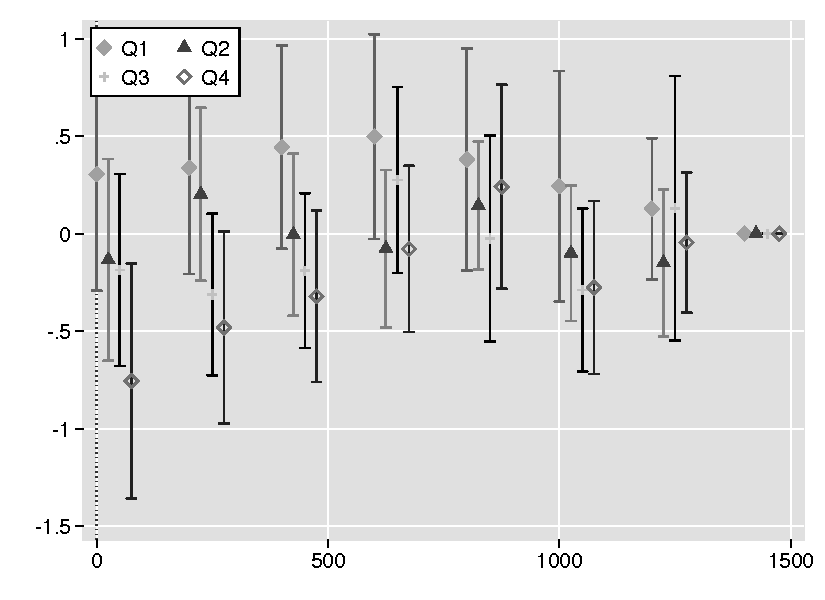
\includegraphics[width=\textwidth,trim={0.3cm .3cm 0.1cm 0cm}, clip=true]{figures/price_dist_3d_no_ctrl_q}
        \end{subfigure}
        \hfill
        \begin{subfigure}[b]{0.48\textwidth}
                    \caption[Network2]%
            {{\footnotesize Distance 3-Diff, purch date/erf controls}}    
            \label{fig:prefor}
            \centering
            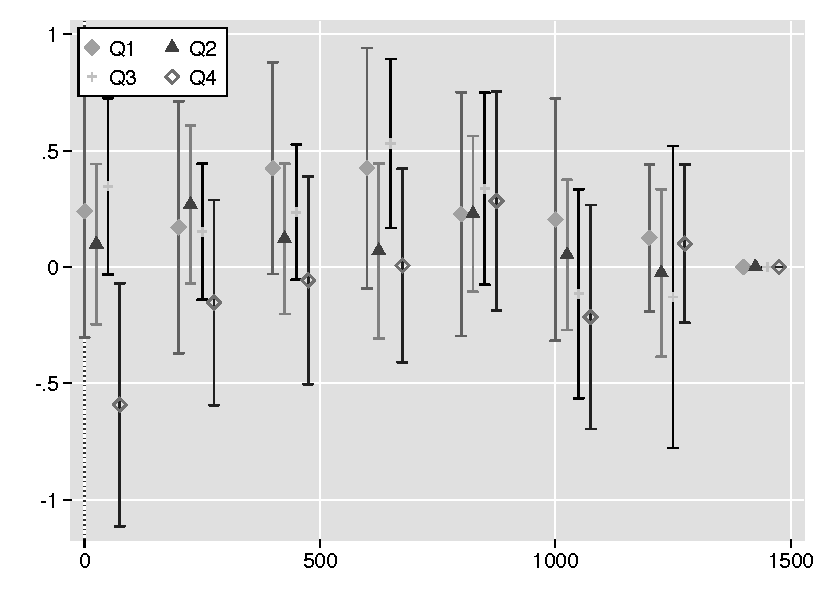
\includegraphics[width=\textwidth,trim={0.3cm .3cm 0.1cm 0cm}, clip=true]{figures/price_dist_3d_ctrl_q}
        \end{subfigure}
        \begin{subfigure}[b]{0.48\textwidth}
                    \caption[Network2]%
            {{\footnotesize Distance 2-Diff}}    
            \label{fig:prefor}
            \centering
            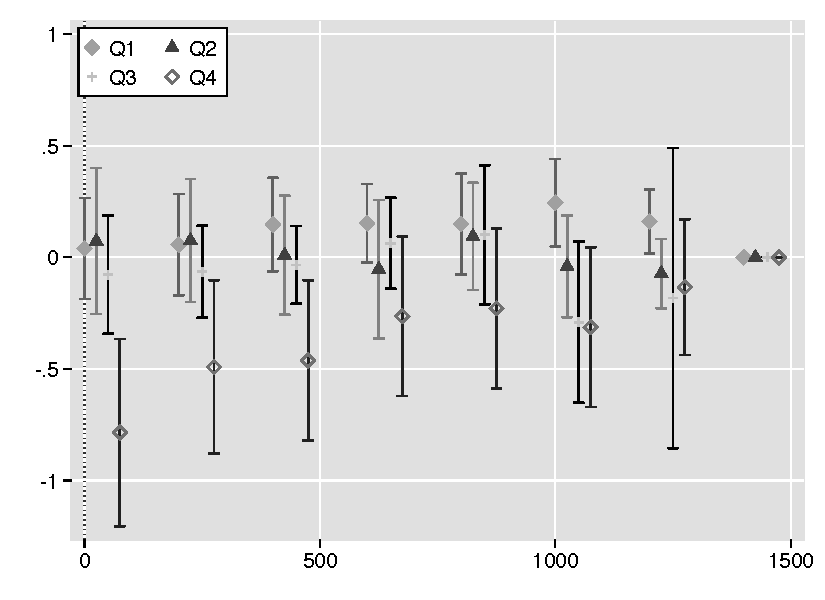
\includegraphics[width=\textwidth,trim={0.3cm .3cm 0.1cm 0cm}, clip=true]{figures/price_dist_2d_no_ctrl_q}
        \end{subfigure}
        \hfill
        \begin{subfigure}[b]{0.48\textwidth}
                    \caption[Network2]%
            {{\footnotesize Distance 2-Diff, purch date/erf controls}}    
            \label{fig:prefor}
            \centering
            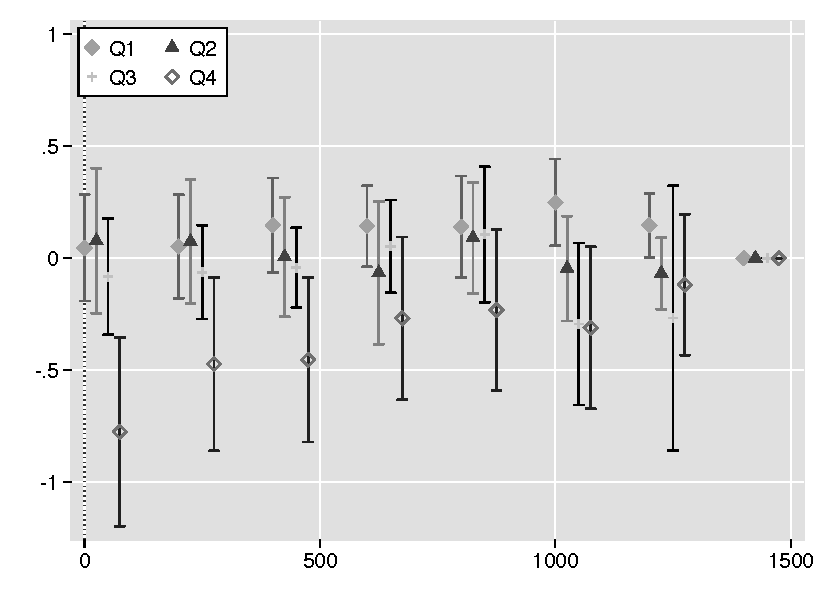
\includegraphics[width=\textwidth,trim={0.3cm .3cm 0.1cm 0cm}, clip=true]{figures/price_dist_2d_ctrl_q}
        \end{subfigure}
       
\end{figure*}


\begin{figure*}
         \centering
   \caption[ Prices over time ]
    {\small Prices over time} 
 \begin{subfigure}[b]{0.48\textwidth}

                    \caption[Network2]%
            {{\footnotesize Time 3-Diff}}    
            \label{fig:prefor}
            \centering
            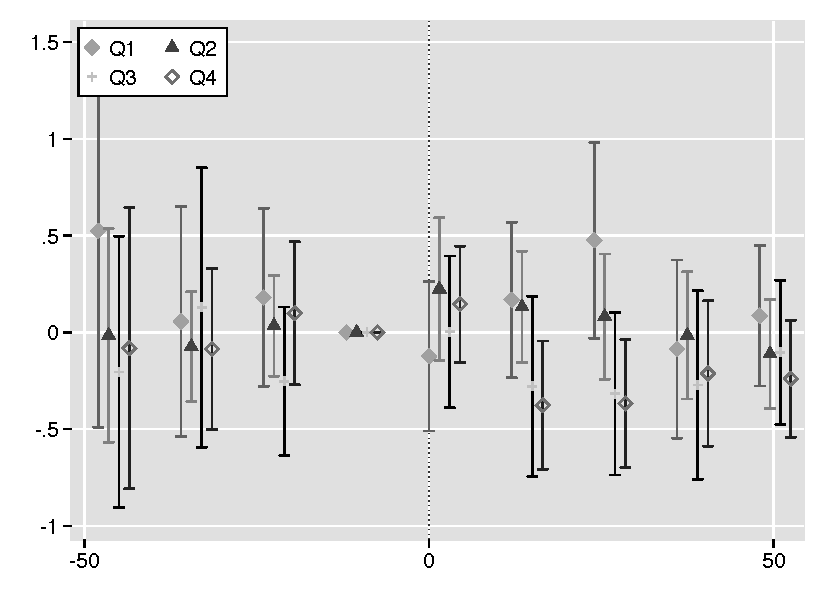
\includegraphics[width=\textwidth,trim={0.3cm .3cm 0.1cm 0cm}, clip=true]{figures/price_time_3d_no_ctrl_q}
        \end{subfigure}
        \hfill
        \begin{subfigure}[b]{0.48\textwidth}
                    \caption[Network2]%
            {{\footnotesize Time 3-Diff, purch date/erf controls}}    
            \label{fig:prefor}
            \centering
            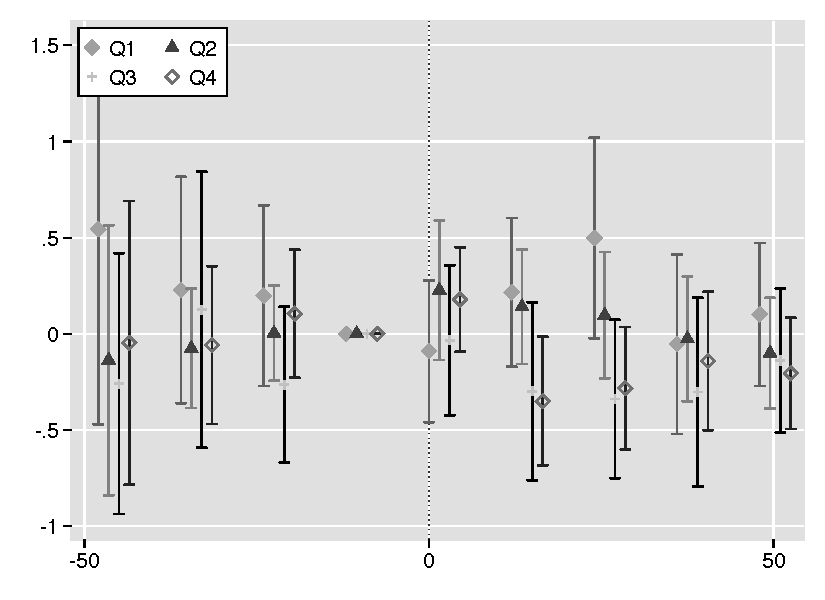
\includegraphics[width=\textwidth,trim={0.3cm .3cm 0.1cm 0cm}, clip=true]{figures/price_time_3d_ctrl_q}
        \end{subfigure}
        \begin{subfigure}[b]{0.48\textwidth}
                    \caption[Network2]%
            {{\footnotesize Time 2-Diff}}    
            \label{fig:prefor}
            \centering
            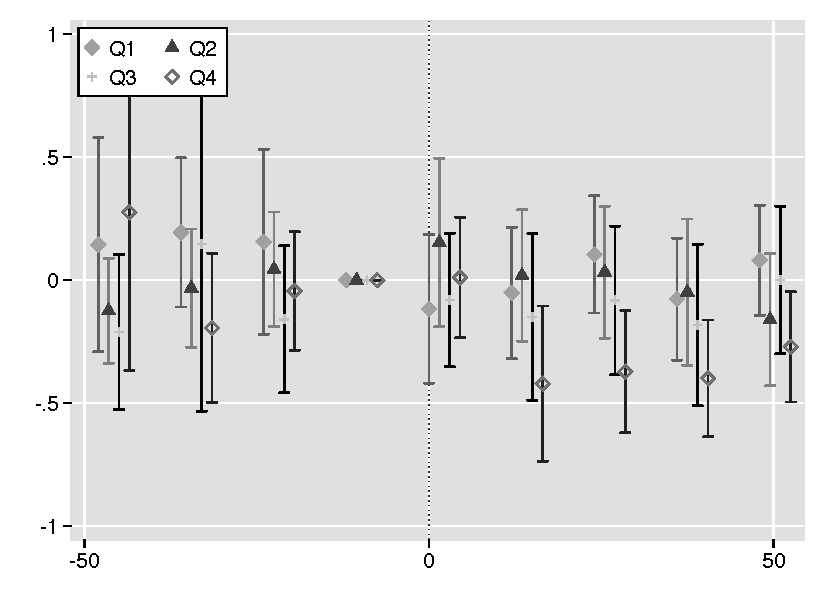
\includegraphics[width=\textwidth,trim={0.3cm .3cm 0.1cm 0cm}, clip=true]{figures/price_time_2d_no_ctrl_q}
        \end{subfigure}
        \hfill
        \begin{subfigure}[b]{0.48\textwidth}
                    \caption[Network2]%
            {{\footnotesize Time 2-Diff, purch date/erf controls}}    
            \label{fig:prefor}
            \centering
            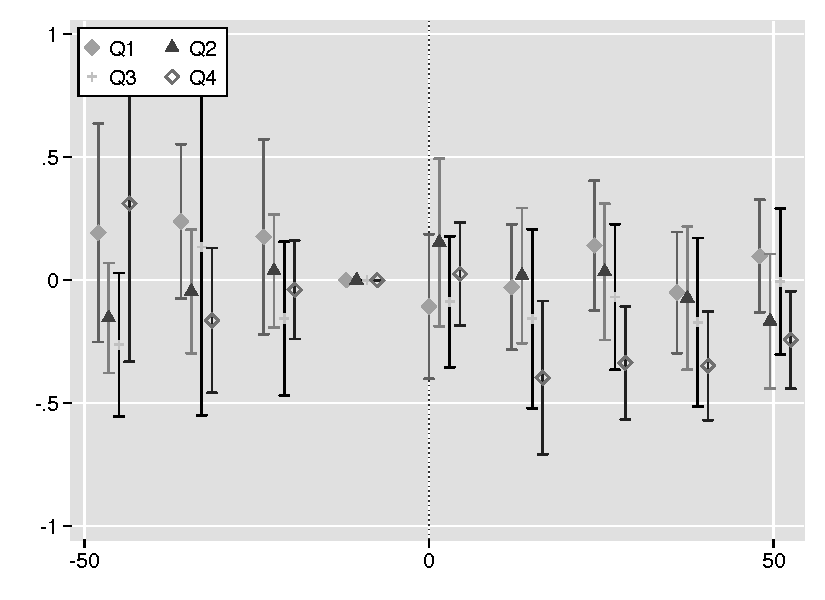
\includegraphics[width=\textwidth,trim={0.3cm .3cm 0.1cm 0cm}, clip=true]{figures/price_time_2d_ctrl_q}
        \end{subfigure}
\end{figure*}


%%%%%%%% TRANSACTION FREQUENCY




\begin{table}
\small
\centering
\caption{Triple Difference Estimates on Transaction Frequency}\label{table:priceDDD_het}
\vspace{-2mm}
\begin{tabular}{lCC}
\toprule
 & \small (1) & \small (2)   \\ \midrule 

 0-500m outside project &      -0.070                   &      -0.075                   \\
                    &     (0.053)                   &     (0.047)                   \\[0.5em]
Lot Size/Year-Month &                               &  \checkmark                   \\
r2                  &        0.01                   &        0.02                   \\
N                   &   2,642,760                   &   2,642,760                   \\

\\
\textbf{By Income Quartile:} \\

 Q1                  &      -1.729\textsuperscript{b}&      -1.639\textsuperscript{b}\\
                    &     (0.699)                   &     (0.779)                   \\[0.3em]
Q2                  &      -1.146                   &      -0.954                   \\
                    &     (0.698)                   &     (0.629)                   \\[0.3em]
Q3                  &      -0.146                   &      -0.126                   \\
                    &     (0.783)                   &     (0.762)                   \\[0.3em]
Q4                  &      -0.521                   &      -0.694                   \\
                    &     (1.043)                   &     (0.916)                   \\[0.3em]
Lot Size/Year-Month &                               &  \checkmark                   \\
Plot Size (up to cubic)&        0.07                   &        0.10                   \\
N                   &     344,916                   &     344,916                   \\


\bottomrule
\multicolumn{3}{l}{\footnotesize Standard errors clustered at the project level in parenthesis.} \\
\multicolumn{3}{l}{ \textsuperscript{c} p$<$0.10,\textsuperscript{b} p$<$0.05,\textsuperscript{a} p$<$0.01 }
\end{tabular}
\end{table}


\begin{table}
\small
\centering
\caption{Diff-in-Diff Estimates on Transaction Frequency}\label{table:priceDD_het}
\vspace{-2mm}
\begin{tabular}{lCC}
\toprule
 & \small (1) & \small (2)   \\ \midrule 

 0-500m outside project &      -0.217                   &      -0.171                   \\
                    &     (0.312)                   &     (0.269)                   \\[0.5em]
Lot Size/Year-Month &                               &  \checkmark                   \\
Plot Size (up to cubic)&        0.07                   &        0.11                   \\
N                   &     208,772                   &     208,772                   \\

\\
\textbf{By Income Quartile:} \\

 Q1                  &      -0.365                   &      -0.282                   \\
                    &     (0.292)                   &     (0.294)                   \\[0.3em]
Q2                  &       0.262                   &       0.302                   \\
                    &     (0.371)                   &     (0.303)                   \\[0.3em]
Q3                  &      -0.578                   &      -0.452                   \\
                    &     (0.737)                   &     (0.700)                   \\[0.3em]
Q4                  &      -0.195                   &      -0.455                   \\
                    &     (1.056)                   &     (0.948)                   \\[0.3em]
Lot Size/Year-Month &                               &  \checkmark                   \\
Plot Size (up to cubic)&        0.08                   &        0.12                   \\
N                   &     208,772                   &     208,772                   \\


\bottomrule
\multicolumn{3}{l}{\footnotesize Standard errors clustered at the project level in parenthesis.} \\
\multicolumn{3}{l}{ \textsuperscript{c} p$<$0.10,\textsuperscript{b} p$<$0.05,\textsuperscript{a} p$<$0.01 }
\end{tabular}
\end{table} 


\begin{figure*}
       \centering
   \caption[ Transaction frequency over distance ]
    {\small Transaction frequency over distance} 
        %\vspace{2mm}
        \begin{subfigure}[b]{0.48\textwidth}
                    \caption[Network2]%
            {{\footnotesize Distance 3-Diff}}    
            \label{fig:prefor}
            \centering
            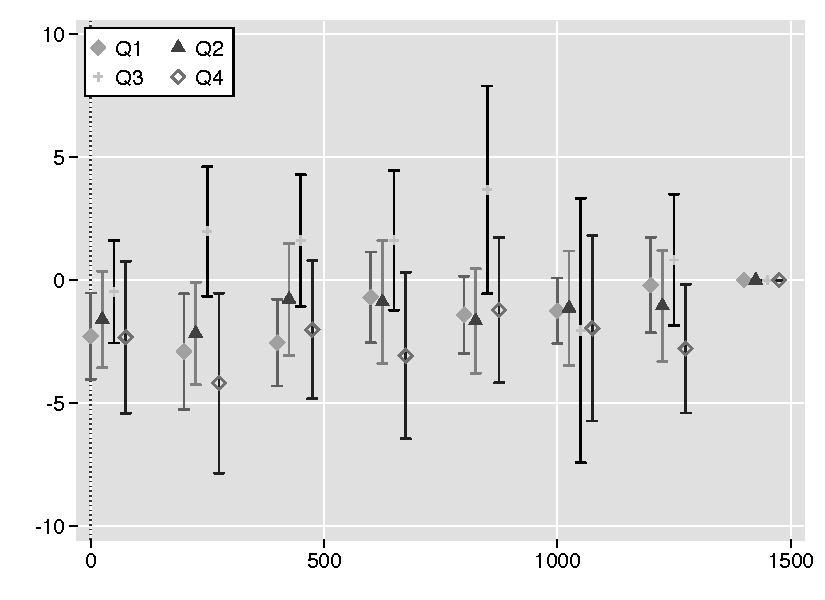
\includegraphics[width=\textwidth,trim={0.3cm .3cm 0.1cm 0cm}, clip=true]{figures/freq_dist_3d_no_ctrl_q}
        \end{subfigure}
        \hfill
        \begin{subfigure}[b]{0.48\textwidth}
                    \caption[Network2]%
            {{\footnotesize Distance 3-Diff, purch date/erf controls}}    
            \label{fig:prefor}
            \centering
            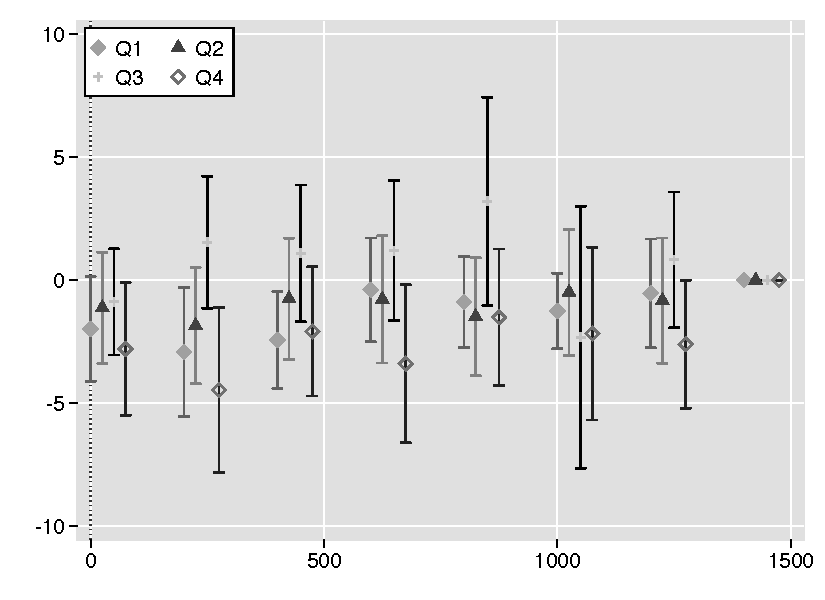
\includegraphics[width=\textwidth,trim={0.3cm .3cm 0.1cm 0cm}, clip=true]{figures/freq_dist_3d_ctrl_q}
        \end{subfigure}
        \begin{subfigure}[b]{0.48\textwidth}
                    \caption[Network2]%
            {{\footnotesize Distance 2-Diff}}    
            \label{fig:prefor}
            \centering
            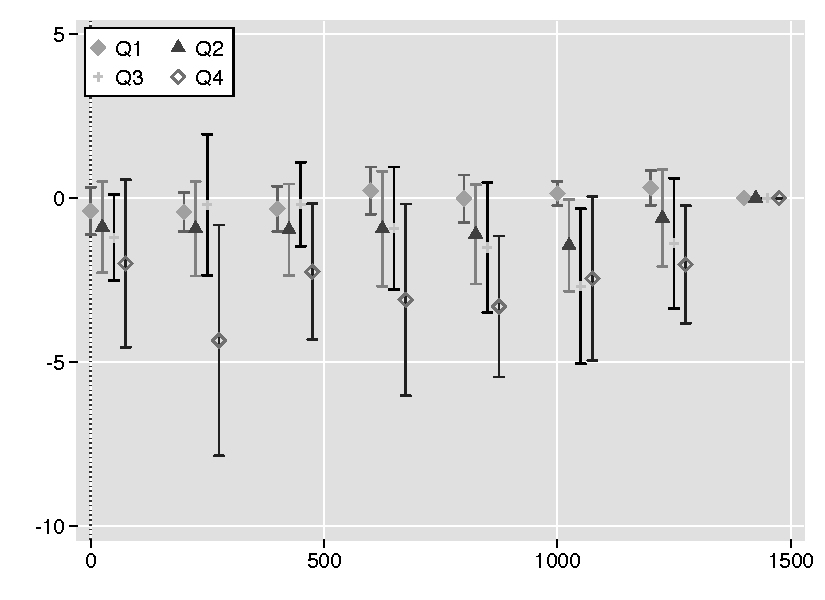
\includegraphics[width=\textwidth,trim={0.3cm .3cm 0.1cm 0cm}, clip=true]{figures/freq_dist_2d_no_ctrl_q}
        \end{subfigure}
        \hfill
        \begin{subfigure}[b]{0.48\textwidth}
                    \caption[Network2]%
            {{\footnotesize Distance 2-Diff, purch date/erf controls}}    
            \label{fig:prefor}
            \centering
            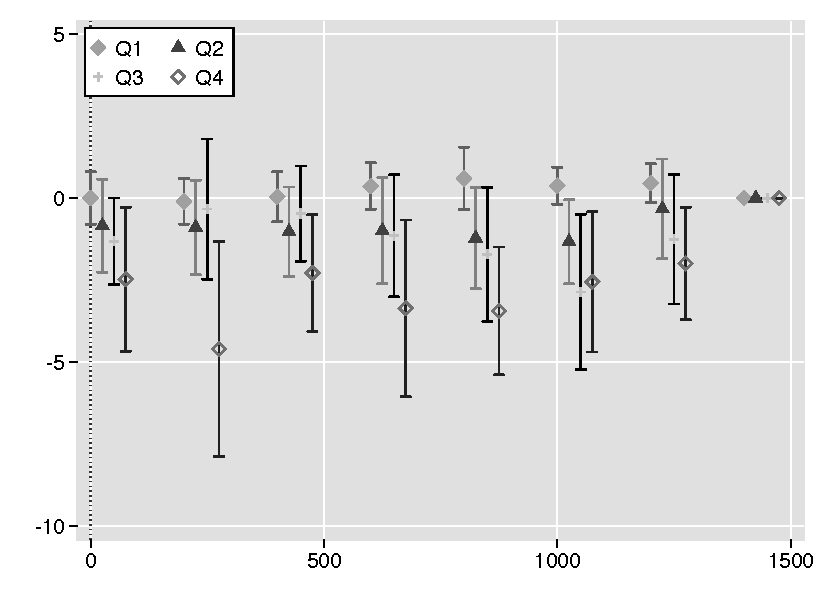
\includegraphics[width=\textwidth,trim={0.3cm .3cm 0.1cm 0cm}, clip=true]{figures/freq_dist_2d_ctrl_q}
        \end{subfigure}
       
\end{figure*}


\begin{figure*}
\centering
   \caption[ Transaction frequency over time ]
    {\small Transaction frequency over time} 
 \begin{subfigure}[b]{0.48\textwidth}
                    \caption[Network2]%
            {{\footnotesize Time 3-Diff}}    
            \label{fig:prefor}
            \centering
            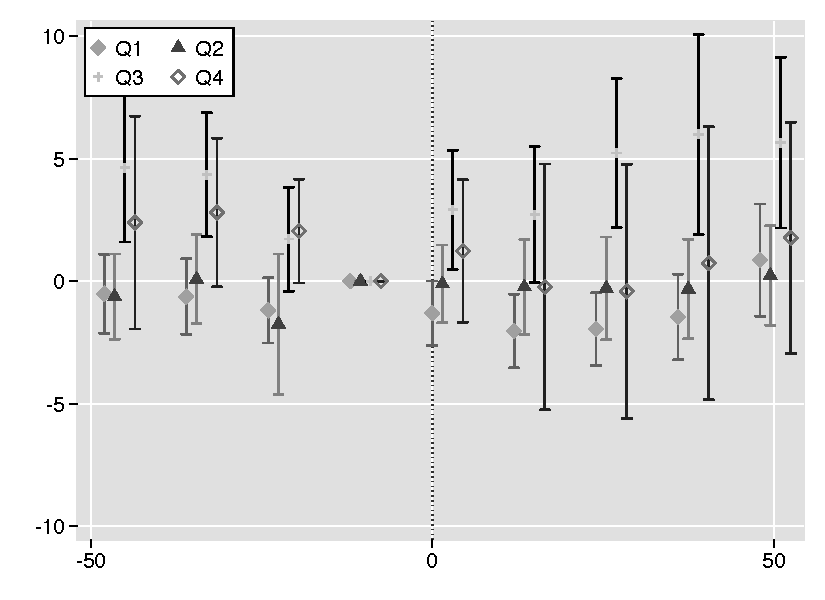
\includegraphics[width=\textwidth,trim={0.3cm .3cm 0.1cm 0cm}, clip=true]{figures/freq_time_3d_no_ctrl_q}
        \end{subfigure}
        \hfill
        \begin{subfigure}[b]{0.48\textwidth}
                    \caption[Network2]%
            {{\footnotesize Time 3-Diff, purch date/erf controls}}    
            \label{fig:prefor}
            \centering
            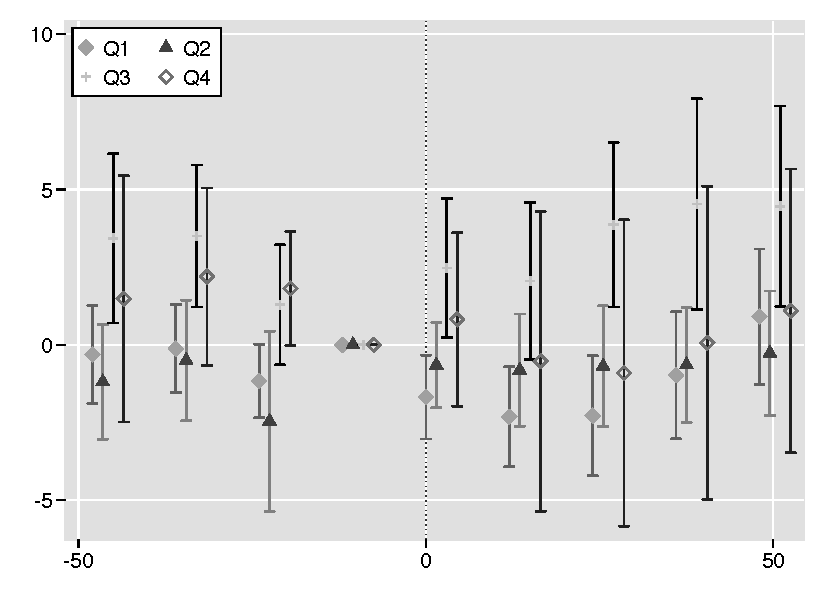
\includegraphics[width=\textwidth,trim={0.3cm .3cm 0.1cm 0cm}, clip=true]{figures/freq_time_3d_ctrl_q}
        \end{subfigure}
        \begin{subfigure}[b]{0.48\textwidth}
                    \caption[Network2]%
            {{\footnotesize Time 2-Diff}}    
            \label{fig:prefor}
            \centering
            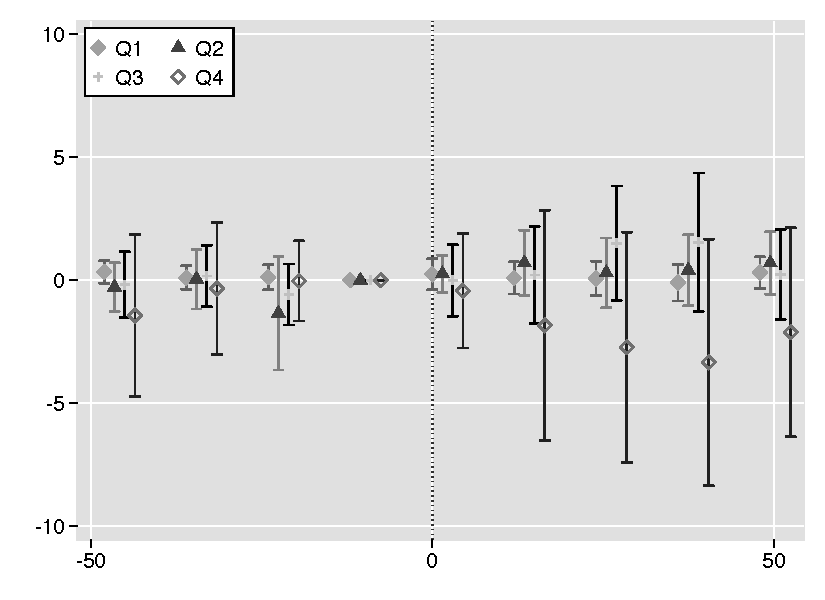
\includegraphics[width=\textwidth,trim={0.3cm .3cm 0.1cm 0cm}, clip=true]{figures/freq_time_2d_no_ctrl_q}
        \end{subfigure}
        \hfill
        \begin{subfigure}[b]{0.48\textwidth}
                    \caption[Network2]%
            {{\footnotesize Time 2-Diff, purch date/erf controls}}    
            \label{fig:prefor}
            \centering
            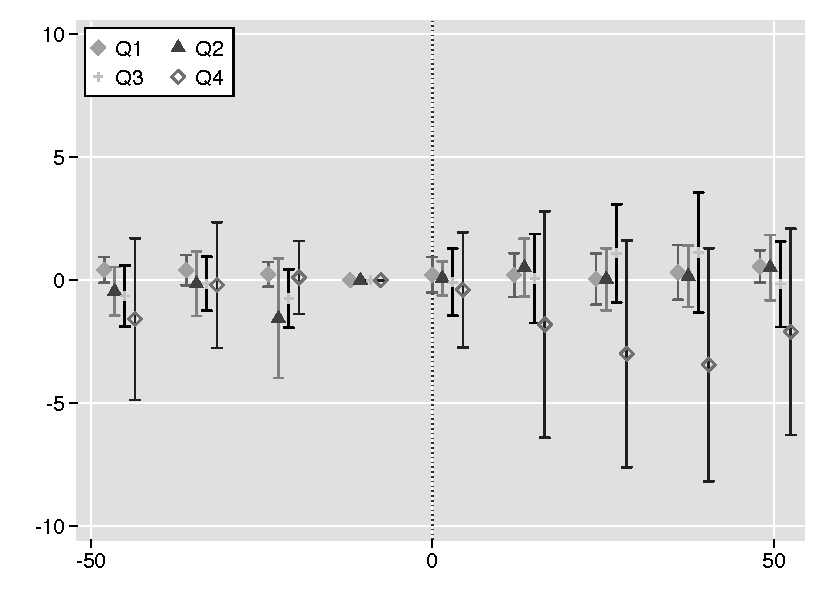
\includegraphics[width=\textwidth,trim={0.3cm .3cm 0.1cm 0cm}, clip=true]{figures/freq_time_2d_ctrl_q}
        \end{subfigure}
\end{figure*}





\begin{table}[h!]
	\centering
	\caption{Housing Comparisons (at endline in constructed areas)}
\vspace{-2mm}
\begin{tabular}{l*{1}{ccccc}}
\toprule
& Proj & \multicolumn{4}{c}{ Spill} \\
&  & Q1 & Q2 & Q3 &Q4 \\
\midrule
Formal House&0.69&0.61&0.69&0.76&0.72 \\
Flush Toilet&0.87&0.68&0.82&0.90&0.88 \\
Piped Water&0.52&0.43&0.53&0.56&0.70 \\
Electricity&0.76&0.71&0.84&0.89&0.85 \\
Total Rooms&3.41&3.34&3.79&3.70&3.97 \\
Own Dwelling&0.38&0.32&0.44&0.46&0.41 \\
HH Size&3.22&2.99&3.17&3.12&2.89 \\
People&7634.99&3436.06&5121.06&5611.31&2151.17 \\
Age HoH&40.56&42.55&43.98&42.48&41.96 \\
African HoH&0.98&0.89&0.88&0.95&0.79 \\
Employed HoH&0.75&0.80&0.79&0.78&0.89 \\
Log HH Income&7.74&7.77&8.01&7.96&8.55 \\
 
\bottomrule
% \multicolumn{4}{l}{\scriptsize ``Constructed'' and ``Unconstructed'' include census small-areas with over 50\% } \\ [-.5em]
% \multicolumn{4}{l}{\scriptsize  area overlap with constructed and unconstructed projects respectively. } \\ [-.5em]
% \multicolumn{4}{l}{\scriptsize ``All''  includes all small-areas.  Means are weighted by land area.}
\end{tabular}
\end{table}



\begin{table}[h!]
	\centering
	\caption{Housing Comparisons Formal Housing Only (at endline in constructed areas)}
\vspace{-2mm}
\begin{tabular}{l*{1}{ccccc}}
\toprule
& Proj & \multicolumn{4}{c}{ Spill} \\
&  & Q1 & Q2 & Q3 &Q4 \\
\midrule
Flush Toilet&0.92&0.80&0.89&0.93&0.90 \\
Piped Water&0.60&0.55&0.64&0.64&0.75 \\
Electricity&0.80&0.80&0.89&0.93&0.88 \\
Total Rooms&3.81&3.87&4.32&4.10&4.24 \\
Own Dwelling&0.43&0.38&0.52&0.53&0.44 \\
HH Size&3.45&3.15&3.46&3.42&2.97 \\
Age HoH&41.97&44.64&46.32&45.11&42.70 \\
African HoH&0.98&0.84&0.86&0.96&0.77 \\
Employed HoH&0.76&0.80&0.80&0.77&0.90 \\
Log HH Income&7.81&7.99&8.15&8.03&8.61 \\
 
\bottomrule
% \multicolumn{4}{l}{\scriptsize ``Constructed'' and ``Unconstructed'' include census small-areas with over 50\% } \\ [-.5em]
% \multicolumn{4}{l}{\scriptsize  area overlap with constructed and unconstructed projects respectively. } \\ [-.5em]
% \multicolumn{4}{l}{\scriptsize ``All''  includes all small-areas.  Means are weighted by land area.}
\end{tabular}
\end{table}





\end{document}


